\begin{document}
%intro

A recent article by SVT Nyheter showed which season is was on the $1^\text{st}$ of November for different areas in Sweden, as can be seen in Fig. \ref{fig:SVT}. According to this article it was already winter in the north of Sweden while in the most south part, including Lund, it was still summer. This did not seem to correspond to what one might observe when looking out the window in Lund, the ground was already covered with red leaves even though it was still summer according to SVT Nyheter. So which definitions of the season are there? Using one of these definitions when do the seasons start in Lund and how does the start of each season vary over a number of years?

\begin{figure}[h!]
\centering
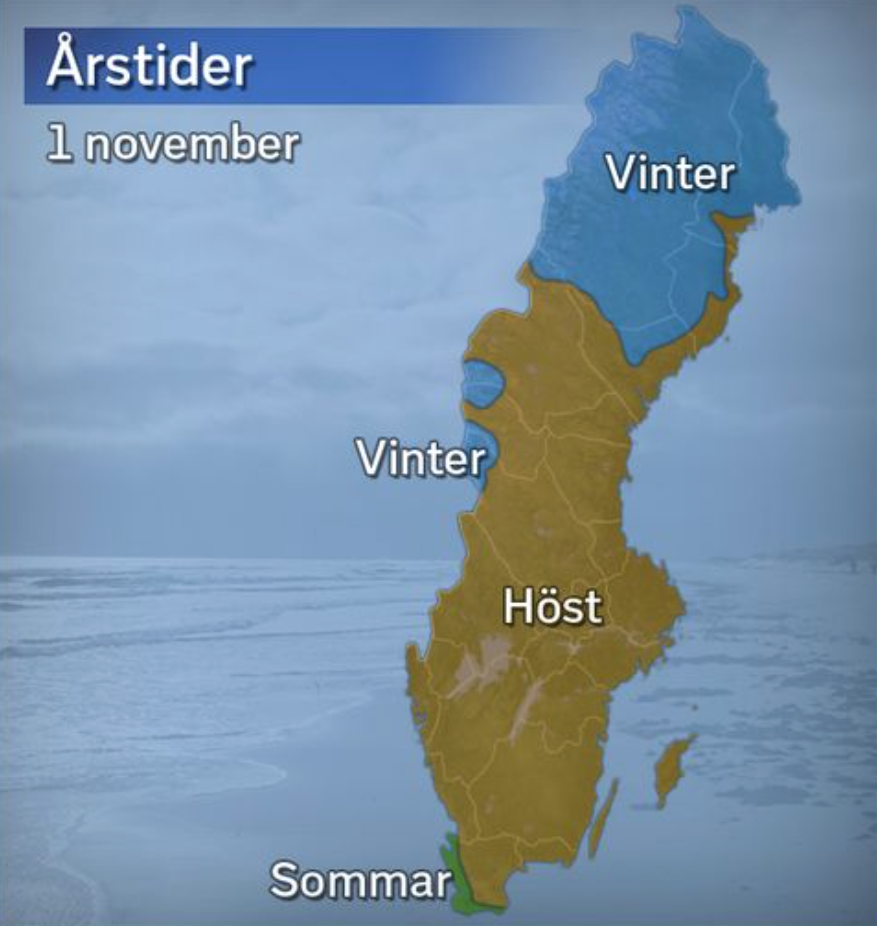
\includegraphics[width=0.4\textwidth]{SVT_seasons.png}
\caption{The season in different areas in Sweden on the $1^\text{st}$ of November. Image from \cite{SVT}.}
\label{fig:SVT}
\end{figure}

\subsection{Definition of the Seasons}
%\cite{SMHI}

There is a definition of the seasons based on the calendar as well as a meteorological definition. According to the definition based on the calendar spring is always from March to May, summer from June to August, fall from September to November and winter from December to February. This is clearly the same for each year and is not dependent on temperature of any other parameter. The meteorological definition of the seasons is based on the average temperature of each day and the seasons can therefore be start on different dates each year. The meteorological winter starts when the average temperature of a day is equal to or below zero for 5 days in a row. The first day of winter is then the first of these 5 days.  The definition for the meteorological summer is similar, but the average temperature needs to be 10 degrees or higher. The meteorological spring starts when the average temperature of a day is between zero and 10 degrees for 7 days in a row. The definition for the meteorological fall is similar, but the temperature only need to be between zero and 10 degrees for 5 days in a row. The season do of course need to occur in the right order, so spring has to start after winter and fall has to start after summer. The meteorological definition of the seasons will be used for the data analyses. 

\subsection{Method}
The temperature data of Lund from Sveriges meteorologiska och hydrologiska institut (SMHI) will be used to determined to beginning of the meteorological season for the years in the dataset.  

%general function:
% - calc start each season
% - make bar graph
% - make histograms 

\begin{figure}[h!]
\centering
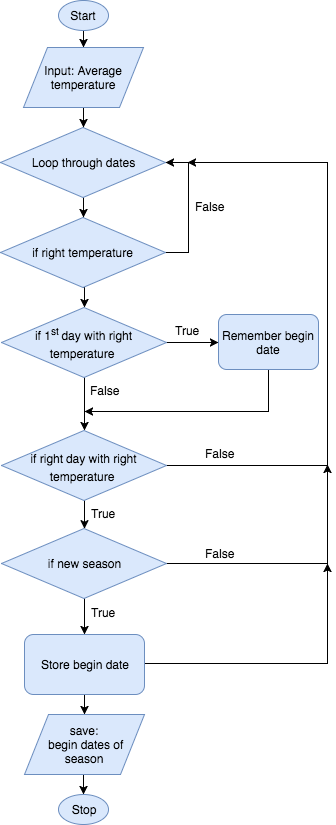
\includegraphics[width=0.4\textwidth]{start_season_diagram.png}
\caption{The code used for the calculation of the start of a season represented in a flowchart.}
\label{fig:flowchart}
\end{figure}
 

\subsection{Results}
%The date is represented by the day of the year (i.e. from 1 to 365 or 366).

\begin{figure}[ht!]
\centering
\subfloat[Bar graph]{\label{fig:spring_bar}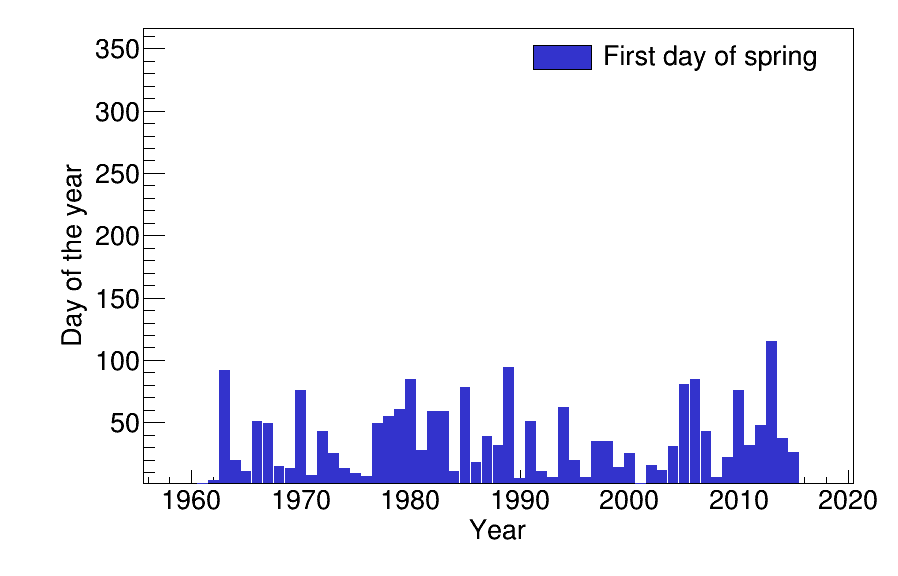
\includegraphics[width=0.5\textwidth]{springStart.png}} 
\subfloat[Histogram]{\label{fig:spring_hist}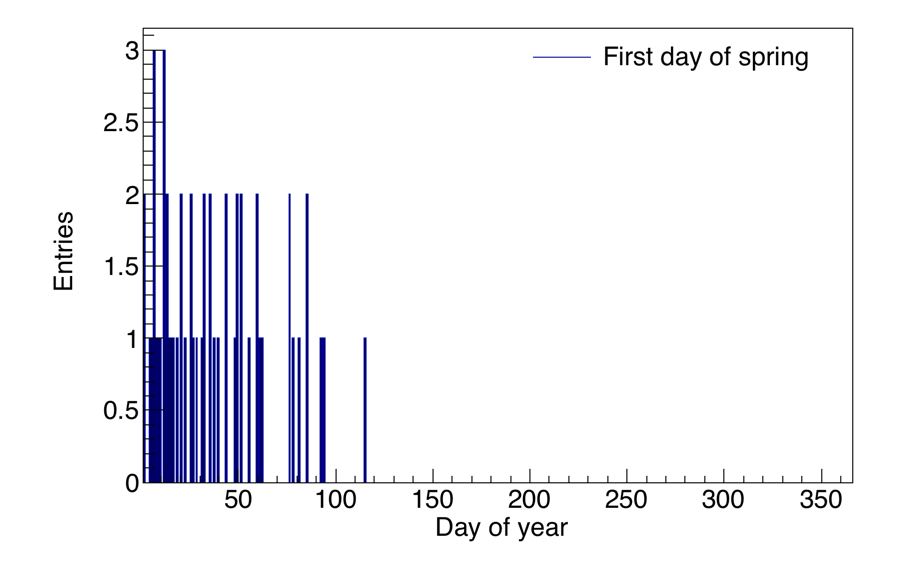
\includegraphics[width=0.5\textwidth]{springHistogram.png}}\\
\caption{The first day on which spring starts for each year in Lund is shown in (a).  While (b) shows the number of times spring starts on a certain day in the year.}
\label{fig:spring}
\end{figure}

\begin{figure}[ht!]
\centering
\subfloat[Bar graph]{\label{fig:summer_bar}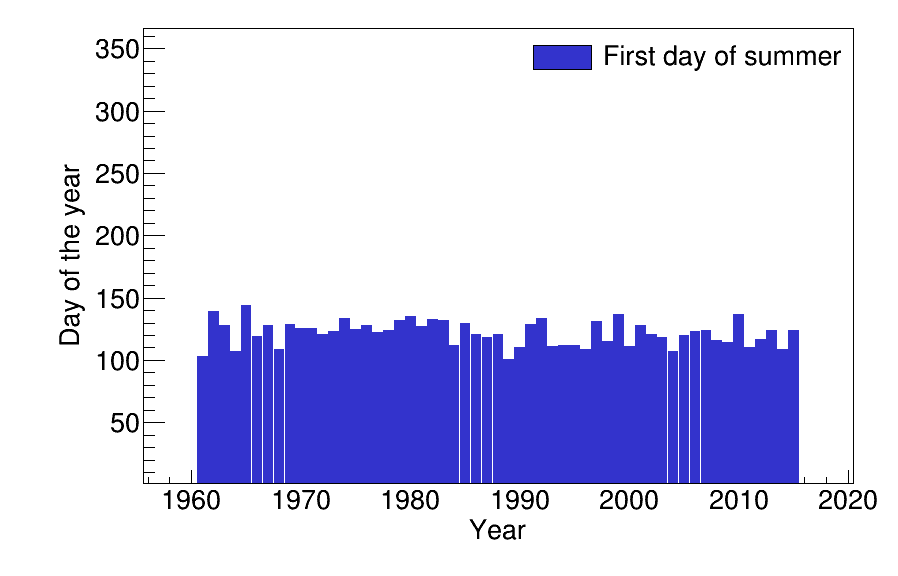
\includegraphics[width=0.5\textwidth]{summerStart.png}} 
\subfloat[Histogram]{\label{fig:summer_hist}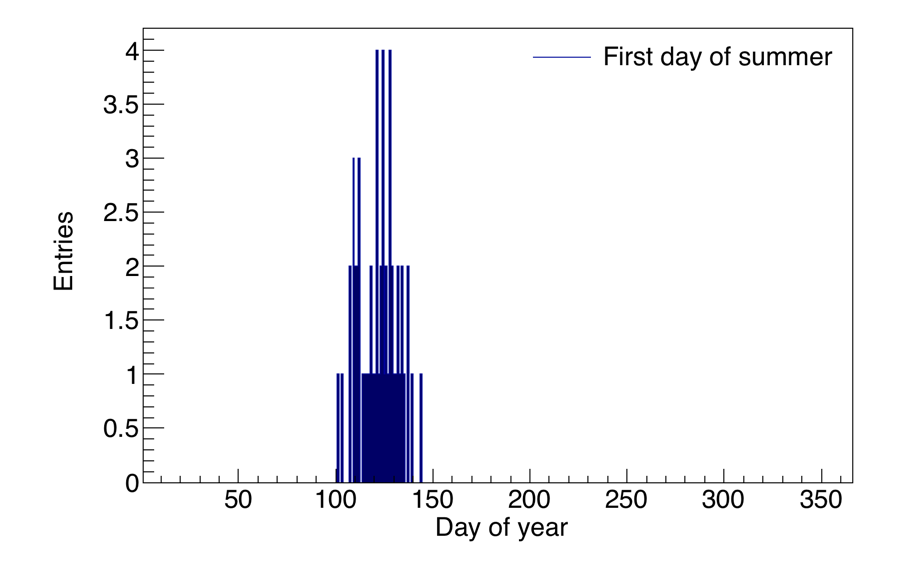
\includegraphics[width=0.5\textwidth]{summerHistogram.png}}\\
\caption{The first day on which summer starts for each year in Lund is shown in (a).  While (b) shows the number of times summer starts on a certain day in the year.}
\label{fig:summer}
\end{figure}

\begin{figure}[ht!]
\centering
\subfloat[Bar graph]{\label{fig:fall_bar}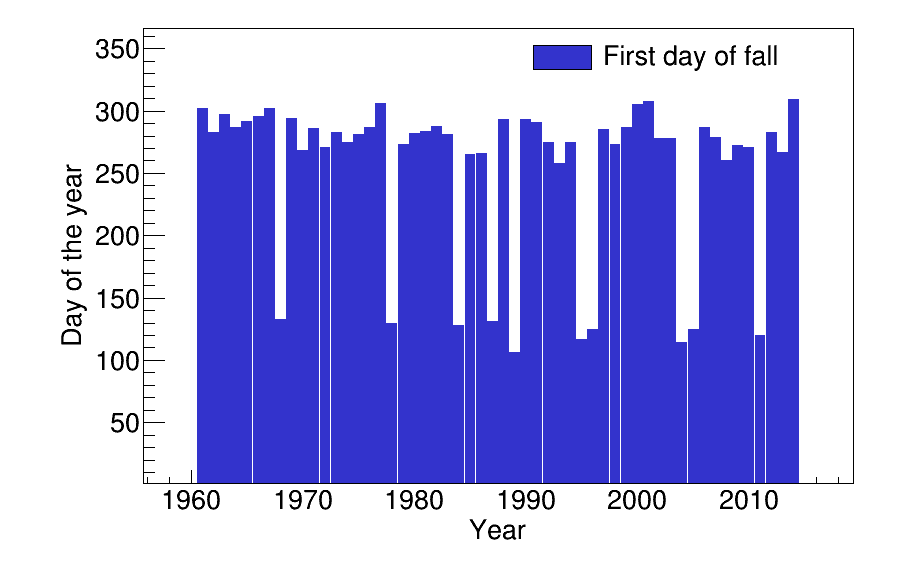
\includegraphics[width=0.5\textwidth]{fallStart.png}} 
\subfloat[Histogram]{\label{fig:fall_hist}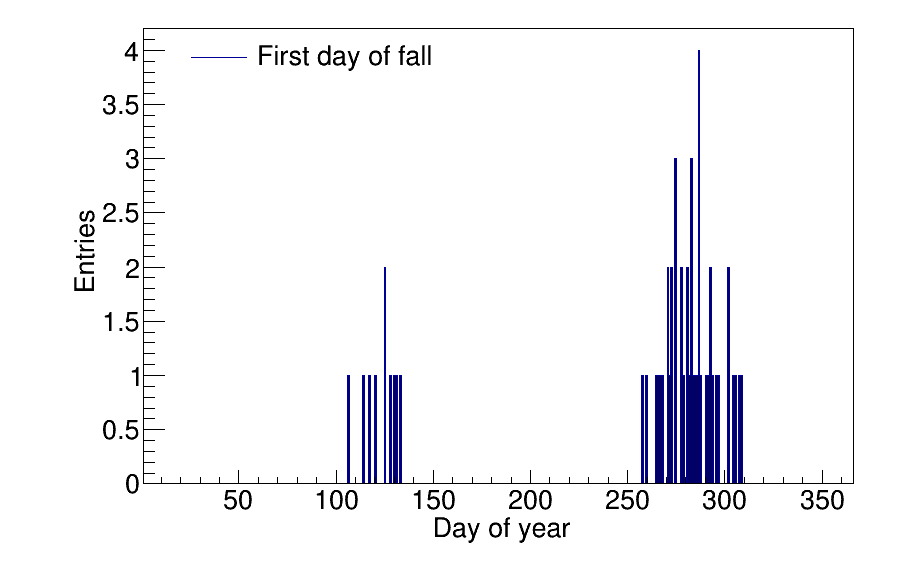
\includegraphics[width=0.5\textwidth]{fallHistogram.png}}\\
\caption{The first day on which fall starts for each year in Lund is shown in (a).  While (b) shows the number of times summer starts on a certain day in the year.}
\label{fig:fall}
\end{figure}

\begin{figure}[ht!]
\centering
\subfloat[Bar graph]{\label{fig:winter_bar}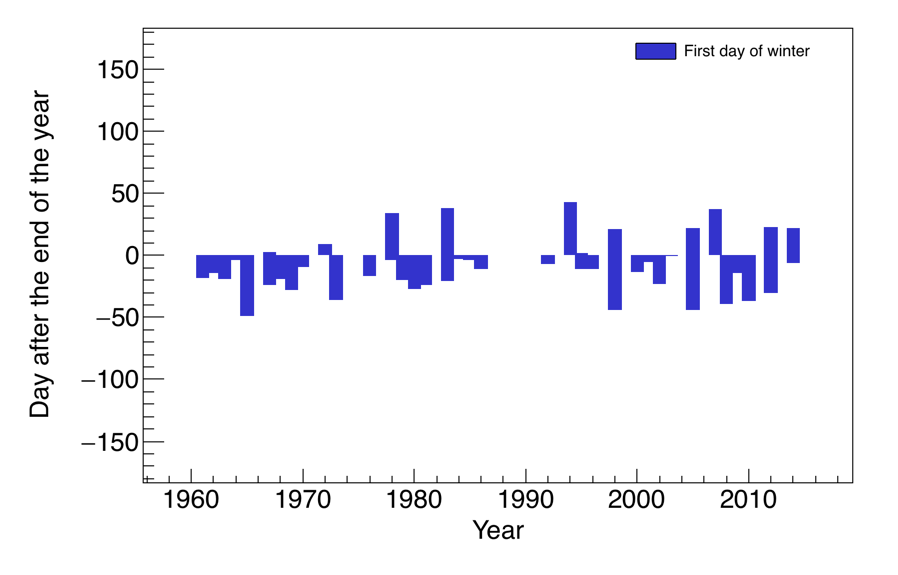
\includegraphics[width=0.5\textwidth]{winterStart.png}} 
\subfloat[Histogram]{\label{fig:winter_hist}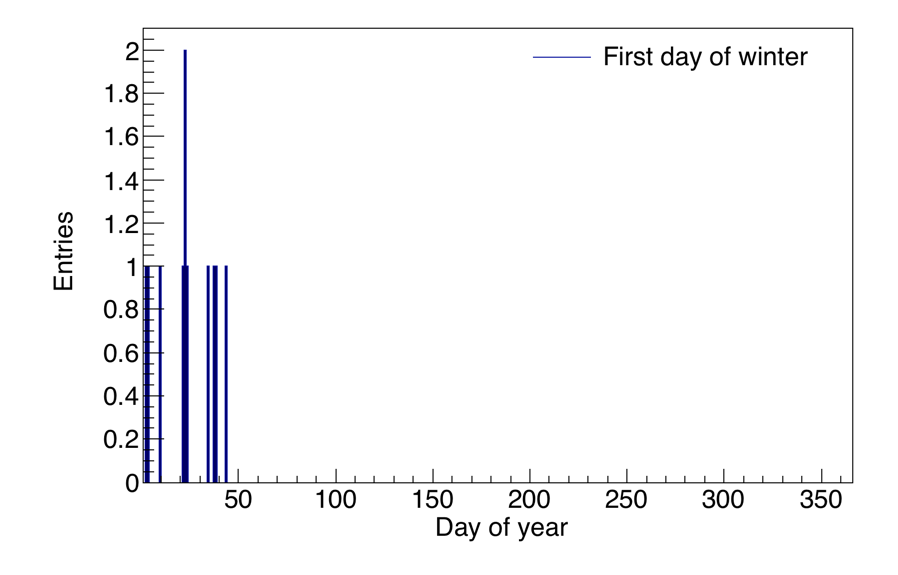
\includegraphics[width=0.5\textwidth]{winterHistogram.png}}\\
\caption{The first day on which winter starts for each year in Lund is shown in (a). The day is given relative to the start of a new year, all negative numbers are before the $1^{\text{st}}$ of January and all the positive numbers are on or after the $1^\text{st}$ of January.  The number of times spring starts on a certain day in the year in given in (b).}
\label{fig:winter}
\end{figure}

\end{document}















